\chapter{Уравнение состояния, излучение и энергия вакуума}

\lectureoverview{История однородной вселенной в значительной степени — это история её масштабного фактора \(a(t)\). Уравнение Фридмана задаёт геометрию, но уравнение состояния вещества определяет, как меняется плотность энергии по мере расширения пространства. Сначала мы выведем \(\rho\propto a^{-3(1+w)}\) из работы, совершаемой жидкостью, затем получим \(P=\rho/3\) для излучения, подсчитывая перенос импульса фотонами, и наконец отождествим энергию вакуума с помощью \(P=-\rho\). Положительная энергия вакуума приводит к расширению де Ситтера; кривизна и знак космологической постоянной порождают решения с отскоком и реколлапсом, которые можно интерпретировать как простые механические системы.}

\section{Масштабный фактор и недостающий закон для вещества}

Сначала восстановим, куда ведёт рассуждение. В рамках однородного и изотропного приближения основная космологическая история закодирована в одной функции, \(a(t)\). Знание этой функции не отвечает на все вопросы о вселенной, но определяет расстояния, скорости расширения и последовательность крупномасштабных эпох. Цель этой лекции пока не в том, чтобы установить эти эпохи по наблюдениям. Она состоит в том, чтобы вывести из основных физических соображений уравнения состояния, которые делают такие модели возможными.

Уже появились две эталонные модели:
\begin{equation}
a(t)\propto t^{2/3}
\qquad\text{(matter domination)},
\end{equation}
и
\begin{equation}
a(t)\propto t^{1/2}
\qquad\text{(radiation domination)}.
\end{equation}
Ни один из этих законов не является точным во все времена. Излучение даёт полезное приближение на ранних временах, а вещество — на более поздних промежуточных; энергия вакуума в конце концов снова меняет поведение на поздних временах. Непосредственный вопрос состоит не в том, как наблюдения выявляют эти эпохи, а в том, что различает соответствующие правые части уравнения Фридмана.

\begin{figure}[htbp]
\centering
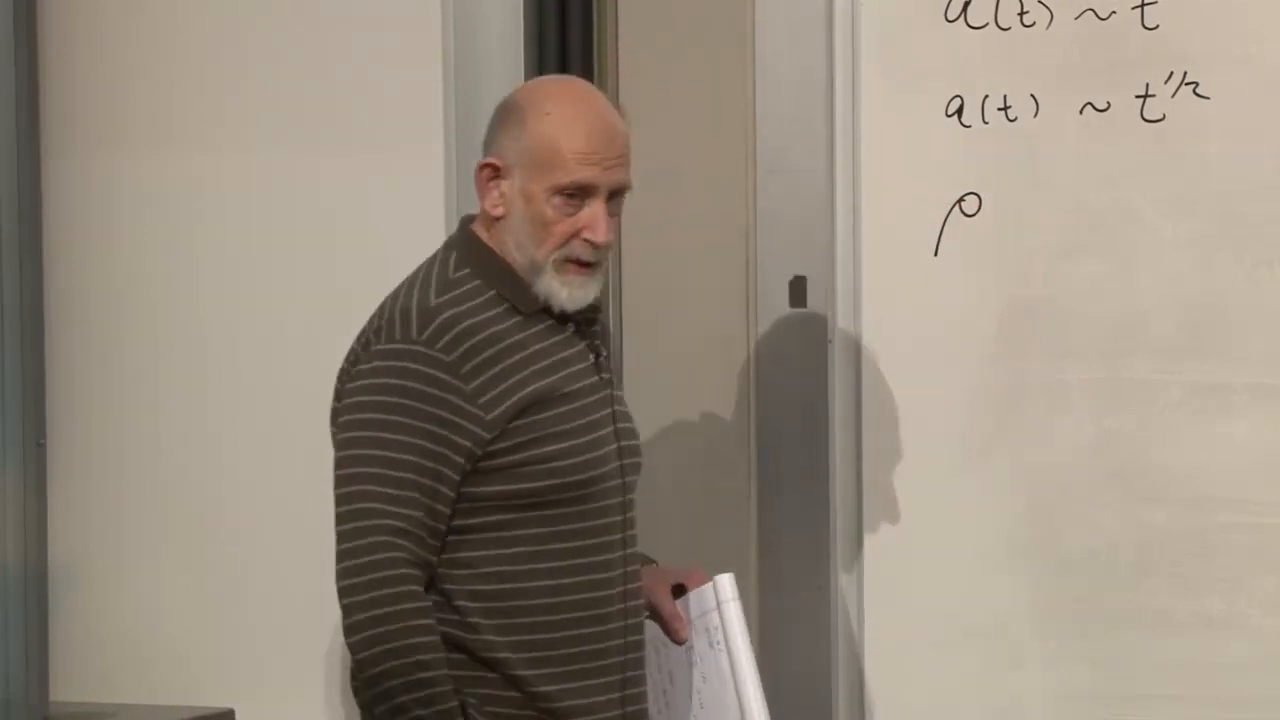
\includegraphics[width=0.72\textwidth]{lecture_05_figure_02.png}
\caption{Рассмотренные степенные законы для масштабного фактора и вновь введённое обозначение плотности. Это переходное состояние доски, а не завершённый вывод.}
\label{fig:c05-review-board}
\lectureframe{00:03:18.380}
\end{figure}

Недостающим звеном является уравнение состояния. Оно определяет, как плотность энергии в правой части уравнения Фридмана меняется с масштабным фактором. Два эталонных закона имеют вид
\begin{equation}
\rho_{\text{matter}}=\frac{\rho_0}{a^3},
\qquad
\rho_{\text{rad}}=\frac{\rho_0}{a^4}.
\label{eq:c05-benchmark-densities}
\end{equation}
Вещество разрежается с объёмом, а объём масштабируется как \(a^3\). Для излучения появляется ещё одна обратная степень \(a\). Мы хотим понять оба правила как следствия соотношения между давлением и плотностью энергии.

\section{От давления к закону масштабирования плотности}

Уравнение состояния в общем случае может включать плотность, давление, температуру и другие переменные. Для космологических компонент, рассматриваемых здесь, примем полезную форму с постоянным \(w\)
\begin{equation}
P=w\rho,
\label{eq:c05-eos}
\end{equation}
где \(w\) характеризует жидкость. На доске используется заглавное \(W\); мы будем использовать общепринятое строчное \(w\). Эта линейная форма охватывает важные случаи ниже, но это упрощающий анзац, а не закон, которому подчиняется всякая возможная жидкость.

Для нерелятивистского вещества плотность энергии определяется главным образом энергией покоя. Если \(n\) — численная плотность, а \(m\) — масса частицы, то схематически
\begin{equation}
\rho\simeq nmc^2.
\end{equation}
Множитель \(c^2\) превращает даже малую массу покоя в огромный запас энергии; полная аннигиляция пылинки высвободила бы макроскопическое количество энергии. Напротив, давление создаётся переносом импульса, когда частицы ударяются о стенку, и имеет порядок \(nmv^2\). Шар для боулинга передаёт больше импульса, чем мяч для пинг-понга, но в холодном газе любая характерная скорость удовлетворяет \(v\ll c\). Следовательно,
\begin{equation}
\frac{P}{\rho}\sim\frac{v^2}{c^2}\ll1,
\qquad
w\simeq0.
\label{eq:c05-dust-eos}
\end{equation}
Излучение движется со скоростью \(c\), так что это приближение к нему неприменимо. Его значение \(w\) мы выведем, а не будем просто предполагать.

Теперь нам нужен общий механизм, который превращает уравнение~\eqref{eq:c05-eos} в закон масштабирования для \(\rho\). Для этого достаточно лабораторного ящика. Галактики, конечно, нельзя буквально поместить в ящик, но в огрублённом описании они ведут себя как частицы, и связь между энергией и давлением можно вывести локально.

\begin{figure}[htbp]
\centering
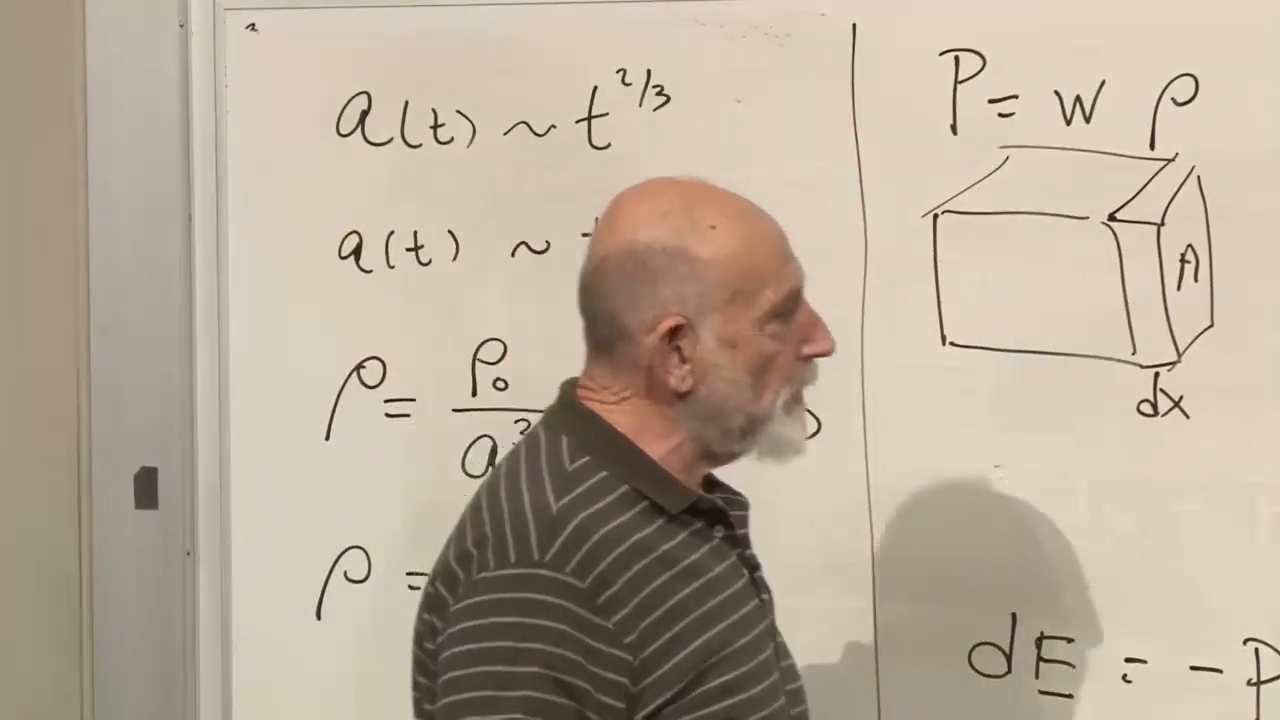
\includegraphics[width=0.86\textwidth]{lecture_05_figure_03.png}
\caption{Уравнение состояния, повторённые законы масштабирования плотности и термодинамический ящик на одной доске. Лектор заслоняет часть прежней записи, поэтому изображение используется ради компоновки и видимых уравнений, а не как полная расшифровка.}
\label{fig:c05-box-board}
\lectureframe{00:13:39.612}
\end{figure}

Левая часть доски содержит повторённые космологические законы масштабирования; правая начинает рассуждение с ящиком. Если читать видимое вместе, содержание связывает
\begin{equation}
\rho_{\text{matter}}=\frac{\rho_0}{a^3},
\qquad
\rho_{\text{rad}}=\frac{\rho_0}{a^4},
\qquad
P=w\rho.
\end{equation}
Наша задача — вывести оба закона для плотности из уравнения состояния.

Одна стенка имеет площадь \(A\). Сдвинем её наружу на \(dx\), так что
\begin{equation}
dV=A\,dx.
\end{equation}
Давление есть сила на единицу площади, поэтому сила, действующая на стенку, равна \(PA\). Газ совершает работу \(PA\,dx=P\,dV\), и энергия, остающаяся внутри, уменьшается.
\begin{equation}
dE=-P\,dV.
\label{eq:c05-work-law}
\end{equation}
\begin{figure}[htbp]
\centering
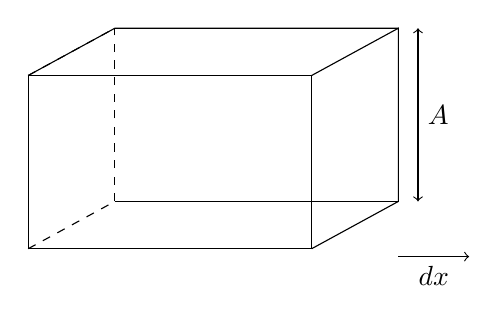
\begin{tikzpicture}[scale=1.0]
\draw (0,0) -- (3.6,0) -- (3.6,2.2) -- (0,2.2) -- cycle;
\draw (3.6,0) -- (4.7,0.6) -- (4.7,2.8) -- (3.6,2.2);
\draw (0,2.2) -- (1.1,2.8) -- (4.7,2.8);
\draw (1.1,0.6) -- (4.7,0.6);
\draw[dashed] (0,0) -- (1.1,0.6);
\draw[dashed] (0,2.2) -- (1.1,2.8);
\draw[dashed] (1.1,0.6) -- (1.1,2.8);
\draw[<->] (4.95,0.6) -- (4.95,2.8);
\node[right] at (4.95,1.7) {\(A\)};
\draw[->] (4.7,-0.1) -- (5.6,-0.1);
\node[below] at (5.15,-0.1) {\(dx\)};
\end{tikzpicture}
\caption{Аккуратная реконструкция термодинамического ящика с площадью грани \(A\) и смещением \(dx\).}
\label{fig:c05-box-redraw}
\end{figure}

Полная энергия равна
\begin{equation}
E=\rho V.
\end{equation}
Дифференцируя, получаем
\begin{equation}
d(\rho V)=\rho\,dV+V\,d\rho.
\end{equation}
Подстановка в уравнение~\eqref{eq:c05-work-law} даёт
\begin{equation}
\rho\,dV+V\,d\rho=-P\,dV.
\end{equation}
Подставим \(P=w\rho\):
\begin{equation}
V\,d\rho=-(1+w)\rho\,dV.
\end{equation}
Этот результат является лишь промежуточным шагом к полезному уравнению, но ещё не им самим. Разделим на \(\rho V\).
\begin{equation}
\frac{d\rho}{\rho}=-(1+w)\frac{dV}{V}.
\end{equation}
\begin{figure}[htbp]
\centering
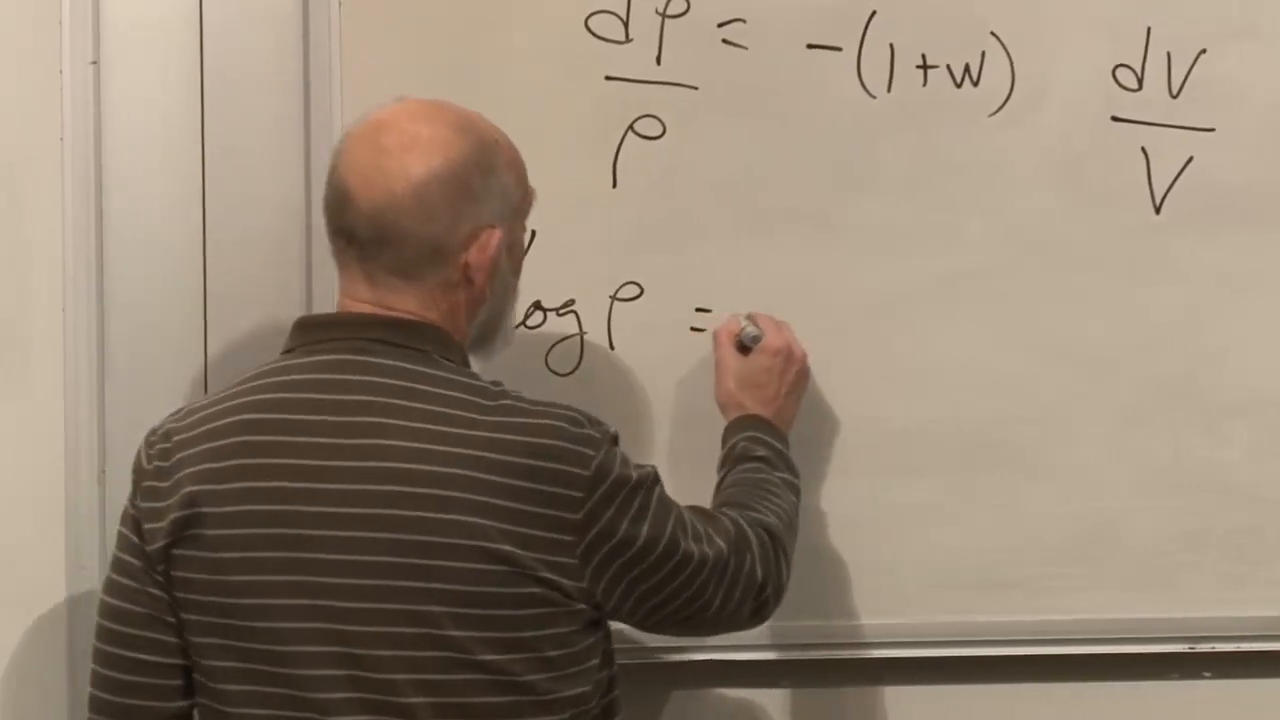
\includegraphics[width=0.78\textwidth]{lecture_05_figure_04.png}
\caption{Разделённое уравнение для плотности и объёма и начало логарифмического интегрирования. Полная правая часть восстановлена по предыдущей алгебре, а не по скрытым пикселям.}
\label{fig:c05-log-board}
\lectureframe{00:15:35.600}
\end{figure}

На кадре показаны разделённое уравнение и начало \(\log\rho=\). Доведём интегрирование прямо до конца:
\begin{equation}
d(\log\rho)=-(1+w)\,d(\log V),
\end{equation}
так что
\begin{equation}
\log\rho=-(1+w)\log V+\text{const.}
\end{equation}
Возводя в экспоненту,
\begin{equation}
\rho\propto V^{-(1+w)}.
\end{equation}
Это и есть закон зависимости плотности от объёма.

Теперь вернёмся от ящика к космологии. Сдвигалась только одна стенка — это был удобный вывод, а не анизотропное предположение. Равномерное расширение по всем трём направлениям даёт то же соотношение для работы, а сопутствующий объём масштабируется как
\begin{equation}
V\propto a^3.
\end{equation}
Следовательно,
\begin{equation}
\boxed{\rho\propto a^{-3(1+w)}}.
\label{eq:c05-density-scaling}
\end{equation}
В \(d\) пространственных размерностях показатель \(3\) заменился бы на \(d\); остальная часть рассуждения не меняется.

\section{Первые приложения: вещество и излучение}

Теперь мы можем восстановить обзорные формулы уже как следствия, а не как предположения.

Для нерелятивистского вещества берём
\begin{equation}
w=0.
\end{equation}
Тогда
\begin{equation}
\rho\propto a^{-3},
\end{equation}
что в точности и есть закон разрежения вещества.

Для излучения пока возьмём
\begin{equation}
w=\frac13.
\end{equation}
Если это верно, то
\begin{equation}
\rho\propto a^{-3(1+1/3)}=a^{-4}.
\end{equation}
Следовательно, дополнительная обратная степень эквивалентна \(w=1/3\). Остаётся вывести это значение из физики фотонов.

\section{Почему давление излучения равно трети его плотности энергии}

Излучение можно описывать как электромагнитные волны или как безмассовые частицы. Воспользуемся фотонами и вычислим давление фотонного газа в ящике. Ящик нарисован в двух измерениях, но газ и его угловое распределение трёхмерны. Фотоны движутся со скоростью света и упруго отражаются от условных стенок.

Пока предположим, что все фотоны имеют одну и ту же энергию \(\epsilon\). Это упрощение исчезнет, когда будут сложены вклады от разных энергий. Пусть \(\vec{\pi}\) — вектор импульса фотона; обычное \(p\) не используется, потому что \(P\) уже обозначает давление. Для безмассовой частицы справедливы соотношения.
\begin{equation}
\epsilon=c\,\pi,
\end{equation}
где \(\pi=|\vec{\pi}|\). В единицах, используемых в лекции, \(c=1\), так что
\begin{equation}
\epsilon=\pi.
\end{equation}
Если \(\nu\) — численная плотность фотонов, то плотность энергии равна
\begin{equation}
\rho=\epsilon\,\nu.
\end{equation}
Пусть ось \(x\) направлена по нормали к одной стенке. За малый интервал \(\Delta t\) фотон, движущийся под углом \(\theta\) к этой нормали, достигает стенки только в том случае, если вначале он находится в слое толщины
\begin{equation}
\Delta x=\Delta t\cos\theta.
\end{equation}
Если он отражается, его \(x\)-компонента импульса меняет знак, так что переданный стенке импульс равен
\begin{equation}
\Delta \pi_x=2\epsilon\cos\theta.
\end{equation}
Сила есть перенос импульса в единицу времени, поэтому одно столкновение даёт вклад \(\Delta \pi_x/\Delta t\). Число фотонов в этом слое равно \(\nu A\Delta x\), но только половина из них движется к стенке, так что учитывать нужно число \(\tfrac12 \nu A\Delta x\). Разделив полную силу на площадь стенки \(A\), получаем
\begin{align}
P(\theta)
&=
\frac{1}{A}
\left(\frac{2\epsilon\cos\theta}{\Delta t}\right)
\left(\frac12 \nu A\Delta x\right) \\
&=
\epsilon\nu\cos\theta\frac{\Delta x}{\Delta t} \\
&=
\epsilon\nu\cos^2\theta \\
&=
\rho\cos^2\theta.
\end{align}
Результат зависит от угла, потому что это лишь вклад фотонов, летящих в одном направлении.

\begin{figure}[htbp]
\centering
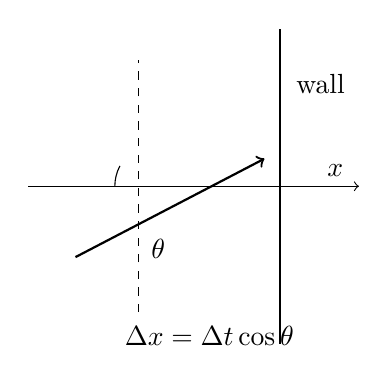
\begin{tikzpicture}[scale=1.0]
\draw[thick] (0,0) -- (0,4);
\draw[->] (-3.2,2) -- (1.0,2);
\node[above] at (0.7,2) {\(x\)};
\draw[dashed] (-1.8,0.4) -- (-1.8,3.6);
\node[below] at (-0.9,0.35) {\(\Delta x=\Delta t\cos\theta\)};
\draw[->,thick] (-2.6,1.1) -- (-0.2,2.35);
\node[below] at (-1.55,1.45) {\(\theta\)};
\draw (-2.1,2) arc[start angle=180,end angle=152,radius=0.55];
\node[right] at (0.08,3.3) {wall};
\end{tikzpicture}
\caption{Импульс фотона, падающего на стенку под углом \(\theta\); геометрия, используемая при выводе давления излучения.}
\label{fig:c05-photon-pressure}
\end{figure}

Усредним по изотропному распределению. Пусть \(\mathbf n=(n_x,n_y,n_z)\) — единичный вектор вдоль направления фотона. Тогда
\begin{equation}
n_x=\cos\theta,
\qquad
n_x^2+n_y^2+n_z^2=1.
\end{equation}
В изотропном газе средние значения \(n_x^2\), \(n_y^2\) и \(n_z^2\) равны. Усредняя приведённое выше тождество, получаем
\begin{equation}
\langle n_x^2\rangle+\langle n_y^2\rangle+\langle n_z^2\rangle=1,
\end{equation}
и по симметрии каждый член одинаков, так что
\begin{equation}
\langle n_x^2\rangle=\langle \cos^2\theta\rangle=\frac13.
\end{equation}
Следовательно,
\begin{equation}
P=\rho\langle \cos^2\theta\rangle=\frac{\rho}{3}.
\end{equation}
Итак, уравнение состояния излучения имеет вид
\begin{equation}
P=\frac13\rho,
\qquad
w=\frac13.
\end{equation}
Множитель \(1/3\) задаётся числом пространственных направлений, между которыми делится квадрат компоненты единичного вектора. В \(d\) изотропных пространственных размерностях тот же аргумент дал бы \(\langle n_x^2\rangle=1/d\). Тем самым завершён обещанный в начале микроскопический вывод.

\subsection{Вопросы для проверки рассуждения об излучении}

\begin{classroomqa}
\audiencequestion{Должны ли все фотоны иметь одинаковую энергию?}
\lecturerresponse{Нет. Выполните вычисление отдельно в каждом интервале энергий. Каждый интервал дает вклад в давление, равный одной трети своей собственной плотности энергии, так что суммирование по спектру сохраняет \(P=\rho/3\). Предположение о равенстве энергий лишь сокращало обозначения. \lecturetimestamp{00:39:08--00:39:36}}
\end{classroomqa}

\begin{classroomqa}
\audiencequestion{Дали бы поглощающие черные стенки тот же ответ, что и идеальные зеркала, и что такое стенка в пустом пространстве?}
\lecturerresponse{Черная стенка в тепловом равновесии поглощает и переизлучает излучение, создавая тот же средний баланс импульса. В космологическом пространстве нет буквальной стенки; поверхность — воображаемая граница. Для каждого фотона, пересекающего ее наружу, изотропия в среднем обеспечивает компенсирующий поток внутрь, поэтому локальное вычисление потока импульса не меняется. Обсуждаемое на лекции излучение — прежде всего тепловое космическое микроволновое фоновое излучение, для которого такая картина равновесия особенно естественна. \lecturetimestamp{00:39:37--00:41:19}}
\end{classroomqa}

\begin{classroomqa}
\audiencequestion{Меняет ли квантовая статистика \(P=\rho/3\)?}
\lecturerresponse{Нет. Бозе-статистика определяет, как фотоны заполняют доступные моды, и тем самым определяет спектр и полную \(\rho\), но изотропное напряжение безмассовых частиц по-прежнему равно одной трети этой плотности энергии. \lecturetimestamp{00:41:51--00:42:02}}
\end{classroomqa}

\begin{classroomqa}
\audiencequestion{А что, если фотоны рассеиваются друг на друге?}
\lecturerresponse{Обычное фотон-фотонное рассеяние чрезвычайно слабо, так что его поправка здесь пренебрежимо мала. При достаточно высокой температуре и плотности столкновения могут рождать электрон-позитронные пары и изменять эффективный состав частиц и уравнение состояния. Это реальный эффект, но он относится к гораздо более горячему режиму, чем тот, который используется в этом рассуждении. \lecturetimestamp{00:42:02--00:43:08}}
\end{classroomqa}

\begin{classroomqa}
\audiencequestion{Куда делась площадь стенки \(A\)?}
\lecturerresponse{Промежуточное произведение — это сила от одного фотона, умноженная на число фотонов, падающих на стенку, а это число пропорционально \(A\). Давление — это сила, деленная на площадь, поэтому окончательное деление сокращает \(A\). Назвать промежуточное выражение давлением слишком рано было упущением в записи на доске; восстановление перехода от силы к давлению это исправляет. \lecturetimestamp{00:43:11--00:44:01}}
\end{classroomqa}

\section{Отрицательное давление и смысл натяжения}

До сих пор частицы ударялись о стенки и толкали их наружу. Эта картина естественным образом приводит к положительному давлению, но ею возможности не исчерпываются.

\begin{classroomqa}
\audiencequestion{Может ли сама плотность энергии быть отрицательной?}
\lecturerresponse{Квантовая теория допускает отрицательные плотности энергии при ограниченных обстоятельствах, а космологическая постоянная формально может иметь любой знак. Такие случаи требуют осторожности и не являются непосредственной отправной точкой. Более привычный путь — отрицательное \emph{давление}, которое может возникать даже при положительной плотности энергии. \lecturetimestamp{00:44:25--00:44:59}}
\end{classroomqa}

\begin{classroomqa}
\audiencequestion{Как давление может быть отрицательным?}
\lecturerresponse{В одномерном мире ящик — это отрезок прямой. Свободно движущиеся частицы отскакивают от его концов и толкают их наружу, создавая положительное давление. Вместо этого соедините концы натянутой струной или пружиной. Если раздвигать концы, пружина тянет их внутрь. Эта направленная внутрь сила есть натяжение, одномерная модель отрицательного давления. \lecturetimestamp{00:45:04--00:46:31}}
\end{classroomqa}

\begin{figure}[htbp]
\centering
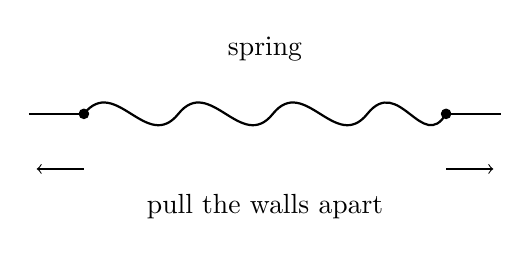
\begin{tikzpicture}[scale=1.0]
\draw[thick] (-3,0) -- (-2.3,0);
\draw[thick] (2.3,0) -- (3,0);
\draw[fill] (-2.3,0) circle (0.06);
\draw[fill] (2.3,0) circle (0.06);
\draw[thick] (-2.3,0)
.. controls (-1.9,0.5) and (-1.5,-0.5) .. (-1.1,0)
.. controls (-0.7,0.5) and (-0.3,-0.5) .. (0.1,0)
.. controls (0.5,0.5) and (0.9,-0.5) .. (1.3,0)
.. controls (1.7,0.5) and (2.0,-0.5) .. (2.3,0);
\draw[->] (-2.3,-0.7) -- (-2.9,-0.7);
\draw[->] (2.3,-0.7) -- (2.9,-0.7);
\node[below] at (0,-0.9) {pull the walls apart};
\node[above] at (0,0.55) {spring};
\end{tikzpicture}
\caption{Одномерная пружина как аналогия отрицательного давления.}
\label{fig:c05-tension}
\end{figure}

Учет работы соответственно меняется. При расширении газ с положительным давлением совершает работу и теряет внутреннюю энергию. Вытягивание наружу против натяжения запасает энергию в пружине. В более общем случае притягивающиеся составляющие могут тянуть друг друга и границу внутрь. Таким образом, система может иметь \(\rho>0\) и \(P<0\), давая \(w<0\), без какого-либо противоречия. Эта возможность принципиальна, поскольку энергия вакуума имеет именно такую комбинацию знаков.

\section{Энергия вакуума и космологическая постоянная}

Энергию вакуума приписывают самому пустому пространству. Квантовая теория поля мотивирует ее через нулевые колебания гармонических осцилляторов, связанных с модами поля, но ее макроскопическое описание не требует, чтобы мы решали эту микроскопическую задачу. Определяющее свойство состоит в том, что пустое пространство имеет одну и ту же плотность энергии, где бы ни выбиралась область и каков бы ни был ее размер.
\begin{equation}
\rho=\rho_0=\text{const.}
\label{eq:c05-vacuum-density}
\end{equation}
Если область объема \(V\) содержит только энергию вакуума, то полная энергия в этой области равна
\begin{equation}
E=\rho_0 V.
\end{equation}
\begin{classroomqa}
\audiencequestion{Меняет ли ящик плотность вакуума, ограничивая допустимые моды поля?}
\lecturerresponse{Полная энергия в конечной области меньше, чем энергия во всем пространстве, потому что объем области меньше; объемная плотность \(\rho_0\) остается той же. Реальные границы могут изменять энергии мод и порождать эффект Казимира, но эта поправка важна, когда расстояния сравнимы с соответствующими длинами волн. Это не та крупномасштабная плотность вакуума, которая используется в космологии. \lecturetimestamp{00:50:06--00:51:25}}
\end{classroomqa}

Введем
\begin{equation}
\Lambda=\frac{8\pi G}{3}\rho_0.
\label{eq:c05-lambda-definition}
\end{equation}
Это определение поглощает комбинацию, возникающую в уравнении Фридмана. Обратное соотношение имеет вид
\begin{equation}
\rho_0=\frac{3\Lambda}{8\pi G}.
\end{equation}
Параметр \(\Lambda\) — это космологическая постоянная. Положительную почти постоянную компоненту, вызывающую позднее ускорение, обычно называют темной энергией.

Зависимость от масштабного фактора уже установлена, так что теперь можно пустить рассуждение с ящиком в обратную сторону, чтобы найти его давление. Поскольку \(d\rho_0=0\),
\begin{equation}
dE=d(\rho_0V)=\rho_0\,dV.
\end{equation}
С другой стороны, термодинамическое соотношение для работы по-прежнему имеет вид
\begin{equation}
dE=-P\,dV.
\end{equation}
Если записать \(P=w\rho_0\), то
\begin{equation}
dE=-w\rho_0\,dV.
\end{equation}
Сравнение дает
\begin{equation}
w=-1.
\end{equation}
и, следовательно,
\begin{equation}
P=-\rho.
\end{equation}
Аналогия с пружиной как раз подготавливала этот знак. Положительная энергия вакуума имеет отрицательное давление; отрицательная энергия вакуума имеет положительное давление. Астрономические измерения \(w\) проверяют, действительно ли компонента на поздних этапах ведет себя как неразбавляющийся вакуум: чем ближе \(w\) к \(-1\), тем ближе поведение к уравнению~\eqref{eq:c05-vacuum-density}.

\begin{classroomqa}
\audiencequestion{Является ли \(P=-\rho\) уравнением состояния пустой Вселенной, и можем ли мы вычислить \(\rho_0\)?}
\lecturerresponse{Это уравнение состояния пустого пространства при наличии энергии вакуума. С его величиной дело обстоит гораздо труднее. Каждое квантовое поле и каждый энергетический масштаб могут давать вклад, включая поля, еще не открытые, поэтому не существует общепринятого вычисления, объясняющего наблюдаемое значение. Главная загадка состоит не в том, как записать \(w=-1\), а в том, почему результирующее \(\rho_0\) столь необычайно мало. \lecturetimestamp{00:57:27--00:58:29}}
\end{classroomqa}

\section{Энергия вакуума в динамике Фридмана}

Выделим энергию вакуума так же, как ранее выделяли чистую материю и чистое излучение. При \(\rho=\rho_0\) уравнение Фридмана принимает вид
\begin{equation}
\left(\frac{\dot a}{a}\right)^2=\Lambda-\frac{k}{a^2},
\label{eq:c05-vacuum-friedmann}
\end{equation}
где \(k=+1,0,-1\) для сферического, плоского и гиперболического пространства. Положительные и отрицательные \(\Lambda\) вместе с тремя вариантами \(k\) дают шесть случаев по знаку, хотя не каждый случай допускает вещественное решение.

\begin{remark}
Здесь используется определение \(\Lambda=(8\pi G/3)\rho_0\), поэтому \(\Lambda\) здесь имеет размерность \(H^2\). В распространенной конвенции \(G_{\mu\nu}+\Lambda_{\mathrm E}g_{\mu\nu}=8\pi G T_{\mu\nu}\) соответствующий параметр равен \(\Lambda_{\mathrm E}=3\Lambda\).
\end{remark}

\subsection{Плоское расширение де Ситтера}

Положим \(k=0\). Тогда
\begin{equation}
\left(\frac{\dot a}{a}\right)^2=\Lambda.
\end{equation}
При \(\Lambda>0\) выберем ветвь расширения:
\begin{equation}
\dot a=\sqrt{\Lambda}\,a,
\end{equation}
и, следовательно,
\begin{equation}
a(t)=C\,e^{\sqrt{\Lambda}\,t}.
\end{equation}
Параметр Хаббла при этом постоянен:
\begin{equation}
H=\frac{\dot a}{a}=\sqrt{\Lambda}.
\end{equation}
Это пространство де Ситтера в плоской нарезке, названное в честь Willem de Sitter, который нашел решение с космологической постоянной вскоре после того, как Einstein ввел этот член в 1917 году. Если \(\Lambda<0\) при \(k=0\), уравнение~\eqref{eq:c05-vacuum-friedmann} не имеет вещественного решения, поскольку \(H^2\) не может быть отрицательным.

\begin{classroomqa}
\audiencequestion{Действительно ли параметр Хаббла здесь постоянен, и есть ли у этого пространства-времени Большой взрыв?}
\lecturerresponse{Для чистого решения в плоской нарезке \(H=\sqrt{\Lambda}\) в точности постоянен. Хотя \(a(t)\to0\) лишь при \(t\to-\infty\), этот координатный участок не геодезически полон: некоторые направленные в прошлое траектории достигают его границы за конечное собственное время. Поэтому сама по себе эта формула не решает глобальный вопрос о Большом взрыве. Полная геометрия де Ситтера содержит больше, чем этот плоский участок; этот вопрос отложен до подробного изучения геометрии. \lecturetimestamp{01:06:54--01:08:07}}
\end{classroomqa}

Схематическое уравнение Фридмана для Вселенной, содержащей материю, излучение, кривизну и энергию вакуума, имеет вид
\begin{equation}
\left(\frac{\dot a}{a}\right)^2
=
\Lambda+\frac{C_m}{a^3}+\frac{C_r}{a^4}-\frac{k}{a^2}.
\label{eq:c05-mixed-friedmann}
\end{equation}
В ранние времена, когда \(a\) мало, доминируют обратные степени, и энергией вакуума можно пренебречь. В поздние времена, когда \(a\) велико, доминирует постоянный член \(\Lambda\). Итак, Вселенная совершает переход: сначала она выглядит как Вселенная с доминированием материи или излучения, а на поздних этапах приближается к поведению типа де Ситтера.

Для экспоненты выполняется \(\ddot a>0\), поэтому доминирование вакуума означает ускоренное расширение. Во время перехода ускорение не обязано быть в точности экспоненциальным, потому что материя все еще вносит вклад в уравнение~\eqref{eq:c05-mixed-friedmann}. Наблюдения на момент чтения лекции описываются как заставшие Вселенную во время этой конкуренции, а не в уже чистой фазе де Ситтера.

\section{Вопросы о вакуумной энергии}

\begin{classroomqa}
\audiencequestion{Если вакуумная энергия — это энергия основного состояния, как она может быть отрицательной?}
\lecturerresponse{Бозонная мода осциллятора даёт вклад \(+\tfrac12\hbar\omega\), тогда как фермионная мода даёт вклад с противоположным знаком. Полная вакуумная энергия представляет собой сумму по многим полям и масштабам, поэтому, пока полное значение не известно, возможен любой знак. Само существование вкладов естественно; трудность состоит в объяснении их чрезвычайно малого остатка. \lecturetimestamp{01:12:00--01:14:12}}
\end{classroomqa}

\begin{classroomqa}
\audiencequestion{Означает ли постоянное \(w=-1\) будущий Большой разрыв?}
\lecturerresponse{Нет. Космологическая постоянная с \(w=-1\) даёт экспоненциальное расширение типа де Ситтера, но не приводит к расходимости за конечное время, называемой Большим разрывом. Этот сценарий относится к гипотетической фантомной компоненте с \(w<-1\), для которой плотность растёт по мере расширения Вселенной. Здесь никакая такая компонента не предполагается. \lecturetimestamp{01:14:13--01:15:50}}
\end{classroomqa}

\begin{classroomqa}
\audiencequestion{Заставила бы точная суперсимметрия вакуумную энергию обратиться в нуль?}
\lecturerresponse{Она может взаимно сократить вклады нулевых колебаний, потому что каждой бозонной степени свободы соответствует фермионная. Однако природа не демонстрирует точной низкоэнергетической суперсимметрии: наблюдаемые бозоны и фермионы не являются партнёрами, вырожденными по массе. Поэтому точное сокращение не объясняет вакуумную энергию в мире, который мы наблюдаем сейчас. \lecturetimestamp{01:15:51--01:16:20}}
\end{classroomqa}

\begin{classroomqa}
\audiencequestion{Каково огромное расхождение между естественной оценкой вакуумной энергии и наблюдаемым значением?}
\lecturerresponse{Универсальные постоянные \(c\), \(\hbar\) и \(G\) определяют планковские единицы. Скорость \(c\) служит пределом для любого сигнала, \(\hbar\) задаёт универсальный масштаб квантовой неопределённости, а \(G\) связывает любую энергию с гравитацией. Из них строятся планковская масса порядка \(10^{-5}\) граммов и планковская длина порядка \(10^{-33}\) сантиметров; отсюда получается планковская плотность энергии — примерно одна планковская энергия на кубическую планковскую длину. В этих единицах наблюдаемая плотность вакуума в лекции приводится как примерно \(10^{-123}\), причём точная степень зависит от соглашения. Загадка состоит в том, почему вклады, которые естественно указывают на куда больший масштаб, оставляют столь малый ненулевой результат. \lecturetimestamp{01:16:21--01:23:12}}
\end{classroomqa}

\begin{classroomqa}
\audiencequestion{Почему физики были удивлены обнаружением ненулевой космологической постоянной, если вакуумные вклады ожидаемы?}
\lecturerresponse{Последовательные улучшения наблюдений раз за разом давали результат, совместимый с нулём. Эта история подпитывала психологическое ожидание, что некоторый неизвестный точный принцип, возможно в будущей теории квантовой гравитации, обеспечивает полную компенсацию. Последующее обнаружение опровергло это ожидание. Удивление отражало десятилетия всё более жёстких нулевых результатов, а не вывод о том, что вакуумная энергия обязана обращаться в нуль. \lecturetimestamp{01:23:14--01:26:05}}
\end{classroomqa}

\begin{classroomqa}
\audiencequestion{Могут ли наблюдения определить, меняется ли тёмная энергия со временем?}
\lecturerresponse{Они не могут исключить резкое изменение в далёком будущем, но могут сравнивать недавнюю историю расширения на протяжении миллиардов лет. Измерение \(w\) или, более общо, \(w(a)\) проверяет, эволюционировала ли плотность в течение этого интервала. В лекции сообщается о тогдашнем ограничении лишь примерно на десятипроцентном уровне; это число носит исторический характер, тогда как непреходящий смысл состоит в том, что \(w=-1\) соответствует неизменной плотности. \lecturetimestamp{01:26:06--01:27:16}}
\end{classroomqa}

\begin{classroomqa}
\audiencequestion{Выглядел бы результат иначе при другом числе пространственных измерений?}
\lecturerresponse{Общая структура сохраняется. В \(d\) изотропных пространственных измерениях у излучения \(w=1/d\), и оно разрежается как \(a^{-(d+1)}\), тогда как лоренц-инвариантная вакуумная энергия по-прежнему имеет \(w=-1\). Численные коэффициенты в уравнении Фридмана меняются с размерностью, но различие между разрежающимися материей и излучением и неразрежающимся вакуумом сохраняется. \lecturetimestamp{01:27:16--01:27:57}}
\end{classroomqa}

\section{Кривизна и механическая аналогия}

\subsection{Положительная кривизна при положительной вакуумной энергии}

Возьмём \(k=+1\) и \(\Lambda>0\):
\begin{equation}
\left(\frac{\dot a}{a}\right)^2=\Lambda-\frac{1}{a^2}.
\label{eq:c05-closed-vacuum}
\end{equation}
Умножая на \(a^2\),
\begin{equation}
\dot a^2-\Lambda a^2=-1.
\label{eq:c05-inverted-oscillator}
\end{equation}
Рассмотрим \(a\) как координату фиктивной частицы. Тогда \(\dot a^2\) — её кинетический член, \(-\Lambda a^2\) — перевёрнутый квадратичный потенциал, а полная энергия равна \(-1\). Физически допустимая ветвь имеет \(a\geq\Lambda^{-1/2}\): вселенная сжимается из большого размера, достигает состояния покоя при минимальном размере и снова расширяется.

Точное решение имеет вид
\begin{equation}
a(t)=\Lambda^{-1/2}\cosh(\sqrt{\Lambda}\,t).
\label{eq:c05-closed-desitter}
\end{equation}
Используя
\begin{equation}
\cosh(\sqrt{\Lambda}\,t)
=
\frac12\left(e^{\sqrt{\Lambda}\,t}+e^{-\sqrt{\Lambda}\,t}\right),
\end{equation}
Эта функция симметрична по времени. При \(t=0\) \(a=\Lambda^{-1/2}\); в обе стороны по времени она растёт экспоненциально. Поэтому замкнутая нарезка демонстрирует сжатие, несингулярный минимум и повторное расширение. Глобально картина отличается от плоской экспоненциальной нарезки, однако обе системы координат покрывают части одной и той же геометрии де Ситтера.

\subsection{Отрицательная космологическая постоянная}

Запишем \(\Lambda=-|\Lambda|\). Если \(k=+1\), то уравнение~\eqref{eq:c05-vacuum-friedmann} имеет отрицательную правую часть при любом \(a\), тогда как \(H^2\geq0\). Вещественного решения ФРУ этого чисто вакуумного типа не существует.

Для \(k=-1\),
\begin{equation}
\left(\frac{\dot a}{a}\right)^2=-|\Lambda|+\frac{1}{a^2}.
\end{equation}
Умножая на \(a^2\),
\begin{equation}
\dot a^2+|\Lambda|a^2=1.
\label{eq:c05-negative-lambda-oscillator}
\end{equation}
Это уравнение энергии гармонического осциллятора. Поскольку \(a\geq0\), один физический полуцикл имеет вид
\begin{equation}
a(t)=\frac{1}{\sqrt{|\Lambda|}}
\sin\!\left(\sqrt{|\Lambda|}\,t\right),
\qquad
0<t<\frac{\pi}{\sqrt{|\Lambda|}}.
\end{equation}
Открытая вселенная начинается при \(a=0\), достигает \(a_{\max}=|\Lambda|^{-1/2}\) и затем приходит к Большому схлопыванию. Следовательно, открытая пространственная геометрия не гарантирует вечного расширения; отрицательная космологическая постоянная может обратить его вспять. Очень большая положительная \(\Lambda\) разорвала бы связанные структуры, тогда как большая отрицательная вызвала бы быстрое повторное схлопывание.

\begin{figure}[htbp]
\centering
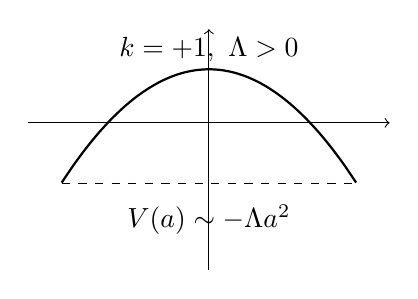
\begin{tikzpicture}[scale=0.85]
\draw[->] (-2.7,0) -- (2.7,0);
\draw[->] (0,-2.2) -- (0,1.4);
\draw[thick,domain=-2.2:2.2,smooth] plot (\x,{-0.35*(\x)^2 + 0.8});
\draw[dashed] (-2.2,-0.9) -- (2.2,-0.9);
\node at (0,-1.45) {\(V(a)\sim -\Lambda a^2\)};
\node at (0,1.1) {\(k=+1,\ \Lambda>0\)};
\end{tikzpicture}
\hspace{2em}
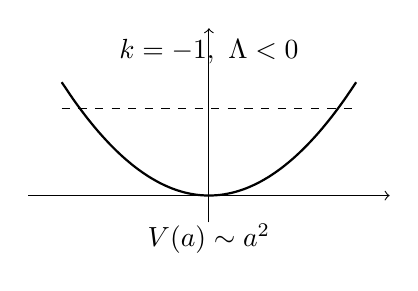
\begin{tikzpicture}[scale=0.85]
\draw[->] (-2.7,0) -- (2.7,0);
\draw[->] (0,-0.4) -- (0,2.5);
\draw[thick,domain=-2.2:2.2,smooth] plot (\x,{0.35*(\x)^2});
\draw[dashed] (-2.2,1.3) -- (2.2,1.3);
\node at (0,-0.65) {\(V(a)\sim a^2\)};
\node at (0,2.15) {\(k=-1,\ \Lambda<0\)};
\end{tikzpicture}
\caption{Схематические эффективные потенциалы для замкнутого де-ситтеровского отскока и открытого повторного схлопывания при отрицательной \(\Lambda\).}
\label{fig:c05-mechanical-potentials}
\end{figure}

\begin{classroomqa}
\audiencequestion{Действительно ли эти уравнения Фридмана — это уравнения Эйнштейна?}
\lecturerresponse{Да. Это уравнение поля Эйнштейна после того, как однородность и изотропия сводят метрику к единственной функции \(a(t)\). Редукция по симметрии устраняет большинство тензорных компонент, оставляя это обыкновенное дифференциальное уравнение для космического расширения. \lecturetimestamp{01:43:52--01:44:05}}
\end{classroomqa}

\begin{classroomqa}
\audiencequestion{Может ли масштабный фактор \(a\) быть комплексным?}
\lecturerresponse{Не в тех вещественных классических ФРУ-космологиях, которые анализируются здесь. Масштабный фактор измеряет пространственный размер и принимается вещественным и неотрицательным. Комплексно продолженные геометрии могут появляться в других математических подходах, но в решениях этой лекции они никакой роли не играют. \lecturetimestamp{01:44:06--01:44:21}}
\end{classroomqa}

\begin{classroomqa}
\audiencequestion{Есть ли физическая причина, по которой давление должно быть линейной функцией плотности?}
\lecturerresponse{Нет. Постоянное \(w\) удобно и как раз описывает основные компоненты, рассматриваемые здесь. Смесь материи, излучения и вакуума не имеет одного постоянного \(w\) во все эпохи, а произвольная среда может иметь нелинейное \(P(\rho)\). Для баротропной жидкости \(dP/d\rho\) задаёт квадрат скорости звука в единицах, где \(c=1\); постоянное \(w\) делает эту производную постоянной, но природа не обязана вести себя именно так. \lecturetimestamp{01:44:21--01:45:34}}
\end{classroomqa}

\section{Что следует запомнить}

Уравнение состояния связывает микроскопическую физику с временной эволюцией масштабного фактора. Адиабатическая работа в сопутствующем объёме даёт
\[
\rho\propto a^{-3(1+w)}.
\]
Для холодной материи \(w=0\) и \(\rho\propto a^{-3}\). Изотропный поток импульса фотонов даёт
\[
\left\langle\cos^2\theta\right\rangle=\frac13,
\qquad
P_{\mathrm r}=\frac{\rho_{\mathrm r}}{3},
\qquad
\rho_{\mathrm r}\propto a^{-4}.
\]

Натяжение делает отрицательное давление физически понятным. Постоянная плотность вакуума удовлетворяет
\[
P_\Lambda=-\rho_\Lambda,
\qquad
w_\Lambda=-1.
\]
Положительная вакуумная энергия даёт экспоненциальное расширение де Ситтера в плоской нарезке и \(\cosh\)-отскок в замкнутой нарезке. Отрицательная вакуумная энергия может заставить снова схлопнуться даже открытую вселенную. При любом знаке уравнение Фридмана можно читать как уравнение эффективной механической энергии. Нерешённый вопрос состоит не в том, почему квантовые поля вносят вклад в вакуумную энергию, а в том, почему их наблюдаемый суммарный вклад почти равен нулю, не будучи в точности нулевым.
